\chapter{Implementation}

This chapter will describe the process of implementing the device --- the commissioning and modification of the computer operating system, the installation of the necessary software and the actual implementation of the program. Any changes to the design of the device will be discussed.

\section{Installing the Operating System}

As mentioned in the design chapter, the appropriate operating system for the Raspberry Pi is Raspberry Pi OS Bullseye 32 bit, partly because of its compatibility with the touchscreen used. The installation is straightforward, using the Raspberry Pi Imager to install the selected system version on the SD card. A Kingston 32 GB SD card was used, although 8 GB would also be sufficient. To get the device working, it is also necessary to provide an internet connection to download the necessary packages, so the device was connected to WiFi. Also, SSH\footnote{Secure shell.} needs to be set up so that the device can be configured remotely when the touchscreen is not yet in use. It should be noted that the system user name must be left \texttt{pi}, otherwise the touchscreen driver installation script does not work correctly. The error is caused by using an absolute path with the user name \texttt{pi} in the installation script, and therefore with a user of a different name the script does not work as it should.   

After successfully uploading the operating system to the SD card, the card was inserted into the device to test its functionality by booting and connecting from a remote computer on the same network.  

\section{Required Packages}

Once the operating system has been successfully commissioned, it is necessary to download the necessary packages to install both the screen driver and the Proxmark software. The following script in Code listing~\ref{code:packages} updates the system and downloads necessary packages.

\begin{lstlisting}[
  caption={~Updating and downloading the necessary packages.},
  label={code:packages},
  language=bash,
  basicstyle=\ttfamily,
  breaklines=true,
  frame=single, 
  keywordstyle=\color{blue},
  commentstyle=\color{green!40!black}, 
  stringstyle=\color{red},
  captionpos=b ]
#! /bin/bash

sudo apt update
sudo apt upgrade
sudo apt install libreadline-dev gcc-arm-none-eabi libssl-dev cmake liblz4-dev libbz2-dev
\end{lstlisting}


\section{Touch Screen Drivers Installation}

After installing the necessary packages, it is necessary to install the driver for the Waveshare LCD 35B-V2 touch screen. This has been performed according to the tutorial in~\cite{waveshare35inch}. Additionally, in Code listing~\ref{code:driver}, the script for installing that driver is provided.

\begin{lstlisting}[
  caption={~Installing the touchscreen driver.},
  label={code:driver},
  language=bash,
  basicstyle=\ttfamily,
  breaklines=true,
  frame=single, 
  keywordstyle=\color{blue},
  commentstyle=\color{green!40!black}, 
  stringstyle=\color{red},
  captionpos=b ]
#! /bin/bash

cd ~
git clone https://github.com/waveshare/LCD-show.git
cd LCD-show/
chmod +x LCD35B-show-V2
./LCD35B-show-V2 # For this specific display, this  LCD35B-show-V2 script must be used
\end{lstlisting}

\section{Proxmark Software Installation}

The Iceman Fork is a very well maintained repository with software for Proxmark devices. This repository on Github~\cite{githubproxmark} will be used for Proxmark software installation.  It contains a client, but also scripts to flash the Proxmark itself.

Using the installation procedure given in~\cite{githubproxmarkdoc}, the software can be installed without any problem. It should be mentioned that before starting the compilation, it is necessary to change the platform in the \texttt{Makefile.platform} configuration file to \texttt{PM3GENERIC}, for which the program will be compiled. It is also necessary to pay attention to the ModemManager, which could damage the device.

\subsection{Flashing Proxmark 3 Easy}

After successful compilation and installation, you can also follow the instructions on Github~\cite{githubproxmarkdoc}. Proxmark 3 Easy can of course also be flashed from a computer other than a Raspberry Pi. 

\section{Operating System Customization}

The following steps are provided to improve the appearance of the software itself, and to create some limitations for users, to have their use of the device limited to the single application:

\begin{itemize}
    \item removing the mouse cursor from the screen,
    \item autostarting the program when the operating system starts,
    \item disabling all unused features such as WiFi or Bluetooth (not done at first for testing purposes).
\end{itemize}

To remove the cursor, the \texttt{/etc/lightdm/lightdm.conf} file needs to be modified, changing \texttt{xserver-command} to \texttt{xserver-command = X -nocursor}. As a result, the cursor is no lonoger visible but the touch screen control works as it should.

Executing the program automatically upon start is done by putting a desktop file in the \texttt{\textasciitilde{}/.config/autostart} folder.


\section{Program Implementation}

This section will explain the principle and description of implementation of the GUI program that controls Proxmark 3 Easy.

\subsection{Architecture}

The implementation followed the design outlined in Chapter~\ref{chap:design}. This means that the \texttt{PyQt5} library allowed for a great layout of individual screens. Thus, each class representing a screen also has a \texttt{QStackWidget} class variable that holds the individual sub-screens.

The program's basic architecture of is depicted in a simplified class diagram in Figure~\ref{fig:classdiagram}. The main class, \texttt{MainWindow}, represents the program window. Then, there are different screens like \texttt{MainScreen}, which contain more screens or other parts of the interface. The implementation also made a great use of class inheritance, where, for example, all screens inherit from one abstract class called \texttt{BaseScreen}. Class inheritance was also used in other cases such as buttons or notification toasts\footnote{A notification toast is a brief, non-interactive alert message that appears temporarily on a mobile device or computer screen, typically in a corner or at the top of the screen.}. This made it easy to create a simple menu in the program. The command execution was implemented as planned in Chapter~\ref{chap:design}.

\begin{figure}[hp]
  \centering
  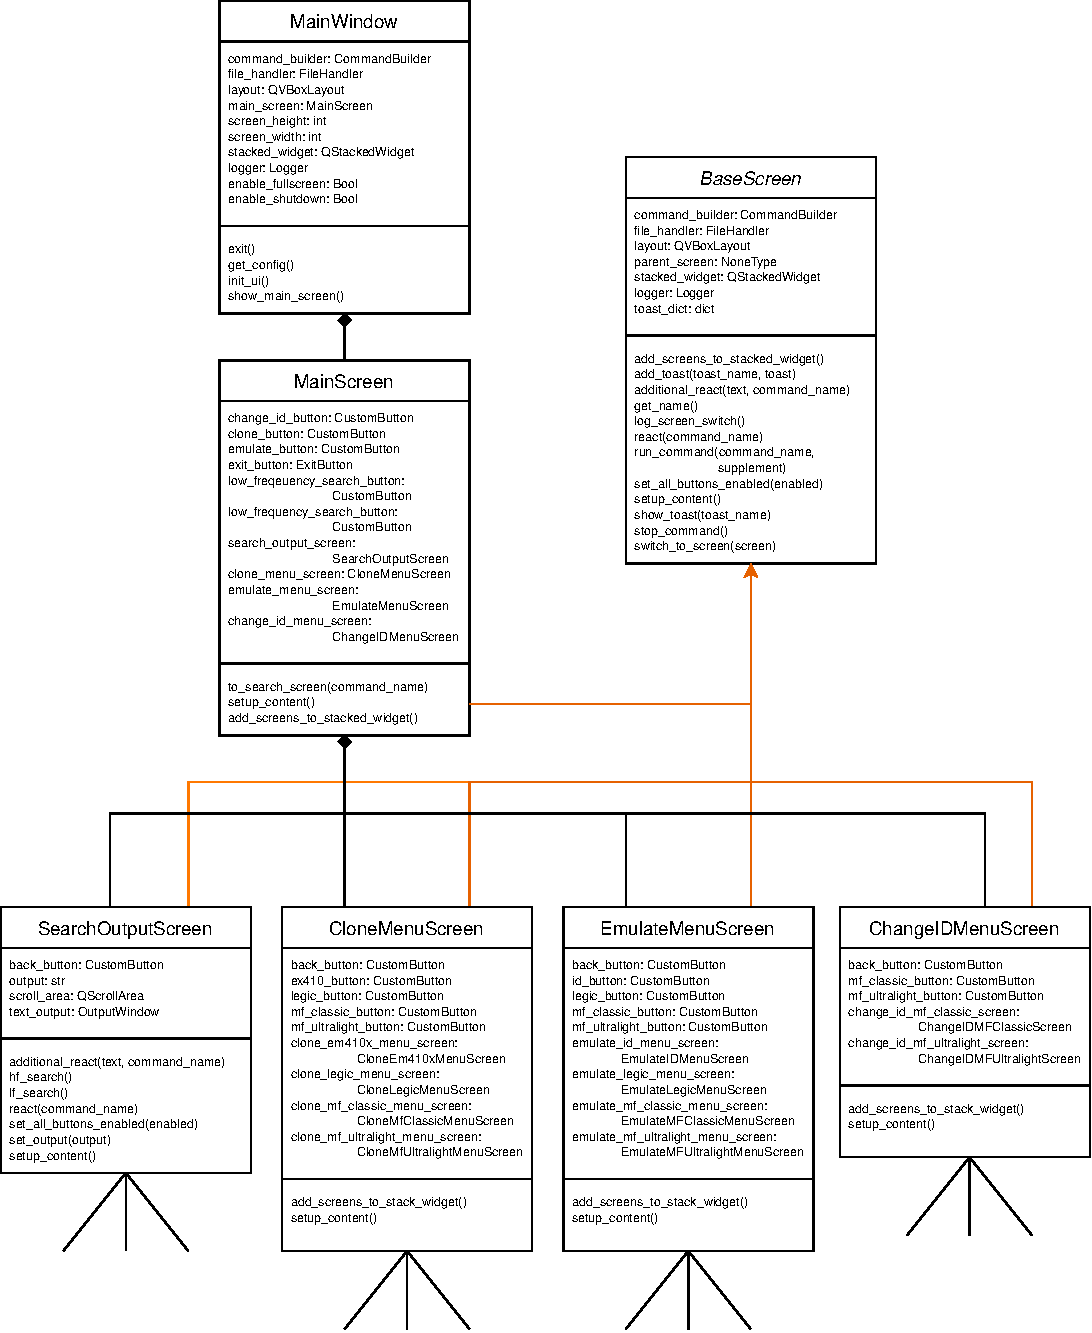
\includegraphics[width=\textwidth]{text/implementation/uml_class_diagram.pdf}
  \caption{~Simplified class diagram describing the GUI part of the software.}
  \label{fig:classdiagram}
\end{figure}

\subsection{Communication With Proxmark}

The program communicates with Proxmark as follows. The Proxmark client has an option to start itself to execute only single command, which when terminated, will terminate the process itself. An example of running the client this way is shown in Code listing~\ref{code:singlecommand}.

\begin{lstlisting}[
  caption={~Starting Proxmark client to execute given command.},
  label={code:singlecommand},
  language=bash,
  basicstyle=\ttfamily,
  breaklines=true,
  frame=single, 
  keywordstyle=\color{blue},
  commentstyle=\color{green!40!black}, 
  stringstyle=\color{red},
  captionpos=b,
  showstringspaces=false]
pm3 -c 'lf search'
\end{lstlisting}

The \texttt{CommandExecutor} class receives individual commands from the \texttt{CommandBuilder} class. These are then started in the \texttt{CommandExecutor} class as a new process, see Code listing~\ref{code:process}. "\textit{The subprocess module allows you to spawn new processes, connect to their input/output/error pipes, and obtain their return codes.}"~\cite{pythonsubprocess}



\begin{lstlisting}[
  caption={~Starting subprocess in Python.},
  label={code:process},
  language=python,
  basicstyle=\ttfamily,
  breaklines=true,
  frame=single, 
  keywordstyle=\color{blue},
  commentstyle=\color{green!40!black}, 
  stringstyle=\color{red},
  captionpos=b ]
process = subprocess.run(command, shell=True, capture_output=True, text=True)
\end{lstlisting}

Then the output of the executed command is passed to the \texttt{OutputHandler} class, which extracts important information from the output depending on the command, e.g. the success rate of execution or some other information like the UID of the tag. This information is then passed to the UI itself. Before each command is executed, the connection of Proxmark 3 Easy to Raspberry Pi is checked. This is done to determine in case of failure exactly why the command was not executed. A simple activity diagram depicting the process of reading and saving a tag information can be seen in Figure~\ref{fig:activitydiagram}.

\begin{figure}[ht]
  \centering
  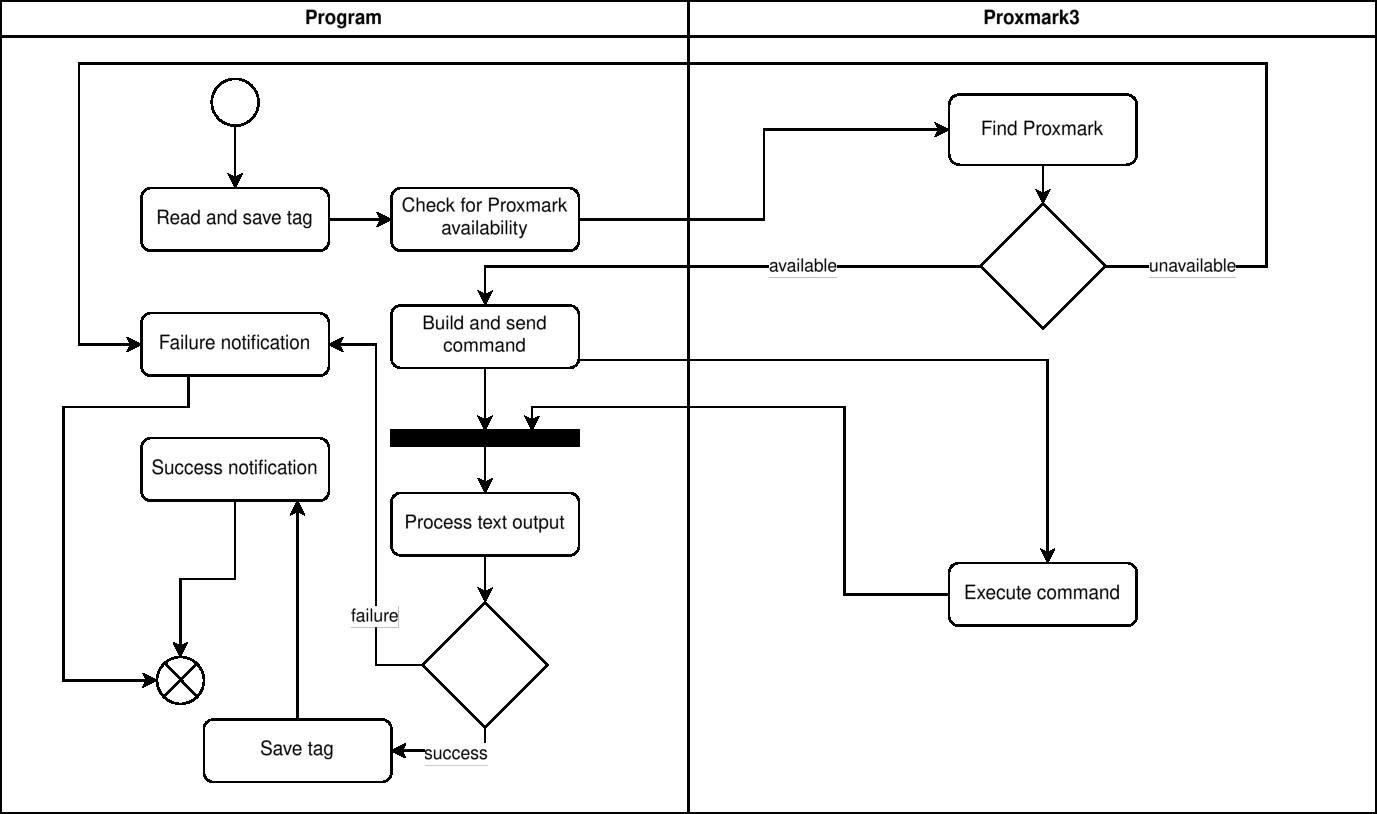
\includegraphics[width=\textwidth]{text/implementation/activity_diagram.pdf}
  \caption{~Simplified activity diagram for reading and saving tag information.}
  \label{fig:activitydiagram}
\end{figure}

\subsection{Graphic User Interface}

The creation of the GUI followed the design presented in the Chapter~\ref{chap:design}. The resulting design is therefore very simple and intuitive. An example of it can be seen in Figure~\ref{fig:ui1}, Figure~\ref{fig:ui2} and Figure~\ref{fig:ui3}.

\begin{figure}[h]
    \centering
    \begin{minipage}[b]{0.315\textwidth}
        \centering
        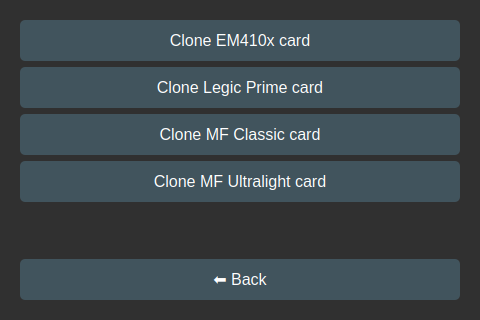
\includegraphics[width=\textwidth]{text/implementation/ui1.png}
        \caption{~Resulting GUI 1.}
        \label{fig:ui1}
    \end{minipage}
    \hfill
    \begin{minipage}[b]{0.315\textwidth}
        \centering
        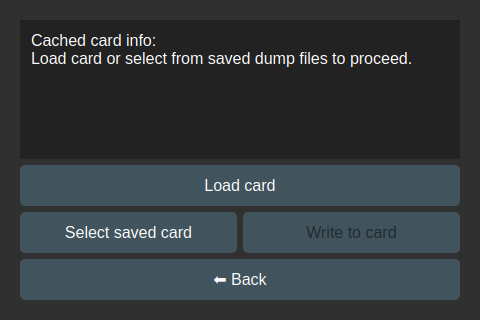
\includegraphics[width=\textwidth]{text/implementation/ui2.png}
        \caption{~Resulting GUI 2.}
        \label{fig:ui2}
    \end{minipage}
    \hfill
    \begin{minipage}[b]{0.315\textwidth}
        \centering
        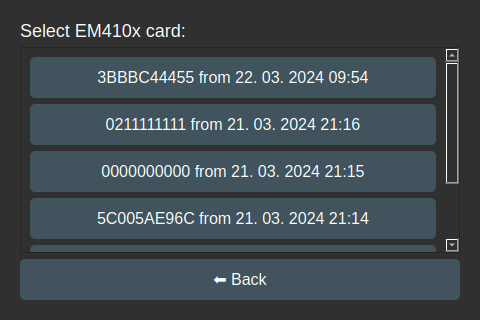
\includegraphics[width=\textwidth]{text/implementation/ui3.png}
        \caption{~Resulting GUI 3.}
        \label{fig:ui3}
    \end{minipage}
\end{figure}


\subsubsection{Feedback to the User}
For a better and more intuitive feeling of use, graphical elements had to be implemented to give the user a kind of feedback that conveys information about, for example, whether the entered command was executed correctly or not, or whether an operation is still in progress.

One of these elements was the blocking of buttons that for some reason should not yet be pressable, e.g. when UIDs are not entered when changing UIDs.

For better feedback to the user, notification toasts were used as a method of user notification. The existing \texttt{pyqt-toast} package available here~\cite{toast} was used. The package license is included in the attachment.


\subsection{User Input}

For input purposes, a custom keyboard containing only the characters 0--9 and A--F was created to edit the UID tag. This option was chosen because it is simpler and more practical than a pop-up keyboard that would already be part of the operating system. The main reason was also to limit input, since the user does not need to and should not be able to enter characters other than those listed above anyway. Another reason for using a custom keyboard was also from a visual point of view. A screenshot of the created keyboard can be seen in Figure~\ref{fig:keyboard}.

\begin{figure}[ht]
  \centering
  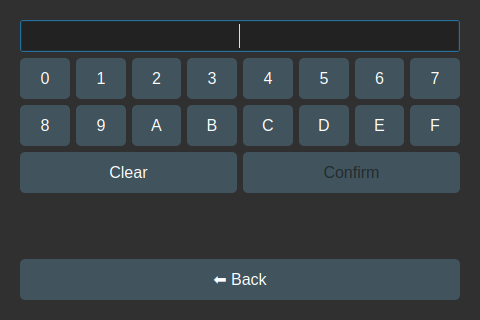
\includegraphics[width=6cm]{text/implementation/keyboard.png}
  \caption{~Screenshot of the created keyboard.}
  \label{fig:keyboard}
\end{figure}


\subsection{Parsing of the Output}

After each command is executed, its output is processed. Since almost every command has different outputs, it was necessary to test all situations, how each command reacts for example to incorrect input or in what form important information appears in the text. 

This is handled by the aforementioned \texttt{OutputHandler} class. An example of how the handling of the output of one of the commands, specifically the \texttt{hf mf autopwn} command, is handled can be seen in Code Listing A. The outputs of other commands were handled in a similar way --- that is, always looking for a particular string in the output. The extraction of other information, here specifically file names from the output, can also be seen in the sample.

\begin{lstlisting}[
  caption={~Processing output of a command in Python.},
  label={code:processingoutput},
  language=python,
  basicstyle=\ttfamily,
  breaklines=true,
  frame=single, 
  keywordstyle=\color{blue},
  commentstyle=\color{green!40!black}, 
  stringstyle=\color{red},
  captionpos=b,
  showstringspaces=false]
def handle_autopwn_mf_card(self):
        dump_file = self.extract_filename_from_backticks("bytes to binary file")
        keys_file = self.extract_filename_from_backticks("Found keys have been")
        if self.contains_sentence("No tag detected"):
            return constants.NO_CARD_FOUND
        if dump_file is None or keys_file is None:
            return constants.PROBLEM
        self.output = (keys_file, dump_file)
        return constants.OUTPUT_HANDLED
\end{lstlisting}
